\chapter{Машинное обучение}
\label{ch:ml}

\section{Кластеризация}
\emph{Кластеризация} — метод обнаружения групп (кластеров) связанных между собой объектов. Кластеризация — пример обучения без учителя.

\subsection{Алгоритм $k$ средних}
Пусть имеется тестовый набор данных $x^{(1)}, \dots, x^{(m)}$, где $x^{(i)} \in \mathbb{R}^n$. Наша цель — выделить $k$ групп из этого набора, где $k$ — предварительно задано. Тогда алгоритм $k$ средних следующий:
\begin{enumerate}
  \item Выбрать случайно центроиды кластеров $\mu^{(1)}, \dots, \mu^{(k)}$, где $\mu^{(i)} \in \mathbb{R}^n$.
  \item Повторять до сходимости (до тех пор, пока центры кластеров не станут постоянными):
    \begin{enumerate}
      \item Для каждого $i$, присвоить \[ c^{(i)} = \operatorname*{arg\,min}_j \| x^{(i)} - \mu_j \|^2. \]
      \item Для каждого $j$, присвоить \[ \mu_j = \frac{\sum_{i = 1}^{m}{1\{ c^{(i)} = j \} x^{(i)}}}{\sum_{i = 1}^{m}{1\{ c^{(i)} = j \}}}. \]
    \end{enumerate}
\end{enumerate}

Этот же алгоритм на пальцах:
\begin{enumerate}
  \item Проинициализировать.
  \item Классифицировать точки по ближайшему к ним центру кластера.
  \item Перевычислить каждый из центров.
  \item Если центры изменились, то повторить с пункта $2$.
\end{enumerate}

Этот алгоритм имеет некоторые недостатки:
\begin{itemize}
  \item Неопределенность с методом выбора начальных центров кластеров.
  \item Количество кластеров надо знать заранее.
  \item Вычислительно сложен.
  \item Качество результата зависит от разбиения, которое в свою очередь завист от выбора начальных центров.
\end{itemize}

\subsection{Метрики}
Нужно уметь вычислять похожесть (расстояние, удалённость) конкретного элемента из набора данных на какой-либо центр. Мы рассмотрим две метрики, используемых в алгоритме $k$ средних. Одна из них — евклидова, другая — коэффициент корреляции Пирсона.

\subsubsection{Евклидова метрика}
Евклидова метрика $d(p, q)$ — это расстояние между двумя точками $p$ и $q$. Пусть $p = (p_1, \dots, p_n)$ и $q = (q_1, \dots, q_n)$, тогда:
\[
d(p, q) = \sqrt{\sum_{k = 1}^n (p_k - q_k)^2}.
\]

В следующей реализации мы возвращаем обратное значение расстояния, так как нужно, чтобы значение для похожих элементов было больше, чем для непохожих. Добавляем же мы единицу в знаменателе для того, чтобы избежать деления на ноль. Квадратный корень не извлекается, так как не важны конкретные значения метрики, а важно то, чтобы соблюдалось правило, что для похожих элементов метрика даёт больший результат, чем для менее похожих.
\begin{pylst}{}{}
from math import sqrt

def sim_distance(vec1, vec2):
    assert len(vec1) == len(vec2)
    sum_of_squares = sum(pow(v1 - v2, 2)
                         for v1, v2 in zip(vec1, vec2))

    return 1 / (1 + sum_of_squares)
\end{pylst}

\subsubsection{Коэффициент корреляции Пирсона}
\emph{Коэффициент корреляции Пирсона} — это мера корреляции двух случайных величин \(X\) и \(Y\). Он принимает значения от \(-1\) до \(+1\), включая концы. Коэффициент определён следующим образом:
\[
\rho_{X, Y} = \frac{cov(X, Y)}{\sigma_X \sigma_Y} = \frac{E[(X - \mu_X)(Y - \mu_Y)]}{\sigma_X \sigma_Y},
\]
где \(cov\) — ковариация, \(E\) — оператор математического ожидания, а \(\mu_X\) и \(\mu_Y\) — среднеквадратичные отклонения.

Этот же коэффициент, но определённый для конкретных выборок и подсчитанный, используя оценки ковариации и среднеквадратичных отклонений:
\begin{align*}
r &= \frac{\frac{1}{n - 1} \sum_{i = 1}^n (X_i - \bar{X})(Y_i - \bar{Y})}{\sqrt{\frac{1}{n - 1} \sum_{i = 1}^n (X_i - \bar{X})^2} \sqrt{\frac{1}{n - 1} \sum_{i = 1}^n (Y_i - \bar{Y})^2}} = \\
  &= \frac{\sum_{i = 1}^n (X_i - \bar{X})(Y_i - \bar{Y})}{\sqrt{\sum_{i = 1}^n (X_i - \bar{X})^2} \sqrt{\sum_{i = 1}^n (Y_i - \bar{Y})^2}},
\end{align*}
где \(\bar{X}\) и \(\bar{Y}\) — средние значения выборок. Они равны \(\frac{1}{n} \sum_{i = 1}^n X_i\) и \(\frac{1}{n} \sum_{i = 1}^n Y_i\), соответственно.

Те же яйца, вид сбоку:
\[
r = \frac{1}{n - 1} \sum_{i = 1}^n \left( \frac{X_i - \bar{X}}{s_X} \right) \left( \frac{Y_i - \bar{Y}}{s_Y} \right).
\]

Можно вывести представить эту формулу так, что алгоритмическая сложность вычисления будет меньше. Учитывая, что
\[
E[(X - \mu_X)(Y - \mu_Y)] = E(XY) - \mu_X \mu_Y,
\]
тогда
\begin{align*}
\rho_{X, Y} &= \frac{E[(X - \mu_X)(Y - \mu_Y)]}{\sqrt{(E[(X - \mu_X)^2])} \sqrt{(E[(Y - \mu_Y)^2])}} = \\
  &= \frac{E(XY) - \mu_X \mu_Y}{\sqrt{(E[X^2] - \mu_X^2)} \sqrt{(E[Y^2] - \mu_Y^2)}}. \\
r &= \frac{\frac{1}{n} \sum_{i = 1}^n{X_i Y_i} - \frac{1}{n^2} \sum_{i = 1}^n{X_i} \sum_{i = 1}^n{Y_i}}{\sqrt{\frac{1}{n}\sum_{i = 1}^n{X_i^2} - (\frac{1}{n}\sum_{i = 1}^n{X_i})^2} \sqrt{\frac{1}{n}\sum_{i = 1}^n{Y_i^2} - (\frac{1}{n}\sum_{i = 1}^n{Y_i})^2}} = \\
  &= \frac{\sum_{i = 1}^n{X_i Y_i} - \frac{\sum_{i = 1}^n{X_i} \sum_{i = 1}^n{Y_i}}{n}}{\sqrt{\sum_{i = 1}^n{X_i^2} - \frac{\left(\sum_{i = 1}^n{X_i}\right)^2}{n}} \sqrt{\sum_{i = 1}^n{Y_i^2} - \frac{\left(\sum_{i = 1}^n{Y_i}\right)^2}{n}}}.
\end{align*}

Предположим, что два критика выставили некоторые оценки различным исполнениям чаконны из партиты №2 для скрипки соло И.С. Баха. Значение коэффициента \(-1\) означает, что критики выставили полностью противоположные оценки: где один оценил исполнение высоко, другой оценил низко, и наоборот. Можно сказать, что между их оценками есть зависимость.

Значение \(1\) означает, что критики оценивают исполнения одинаково, но каждый по своей шкале. Так если было три исполнения, и первый критик выставил оценки \([1, 2, 3]\), а второй критик выставил — \([1, 3, 5]\), то всё-равно коэффициент Пирсона будет равен единице.

Значение \(0\) означает, что зависимости в выставлении оценок у критиков нет.
\begin{table}[h!]
  \caption{Интерпретация значений}
  \begin{center}
    \begin{tabular}{lll}
      \toprule
      \textbf{Корреляция} & \textbf{Отрицательный} & \textbf{Положительный} \\
      \midrule
      Нет     & \texttt{[-0.09; 0.0]} & \texttt{[0.0; 0.09]} \\
      Малая   & \texttt{[-0.3; -0.1]} & \texttt{[0.1; 0.3]} \\
      Средняя & \texttt{[-0.5; -0.3]} & \texttt{[0.3; 0.5]} \\
      Большая & \texttt{[-1.0; -0.5]} & \texttt{[0.5; 1.0]} \\
      \bottomrule
    \end{tabular}
  \end{center}
\end{table}

\begin{pylst}{Функция вычисления коэффициента Пирсона}{}
def sim_pearson(vec1, vec2):
    assert len(vec1) == len(vec2)

    n = len(vec1)
    if n == 0:
        return 0

    sum1, sum2 = sum(vec1), sum(vec2)
    sum1_of_squares = sum(pow(v, 2) for v in vec1)
    sum2_of_squares = sum(pow(v, 2) for v in vec2)
    sum_of_products = sum(v1 * v2 for v1, v2 in zip(vec1, vec2))

    num = sum_of_products - (sum1 * sum2 / n)
    den = sqrt((sum1_of_squares - pow(sum1, 2) / n) *
               (sum2_of_squares - pow(sum2, 2) / n))

    if den == 0:
        return 0

    r = num / den
    return r
\end{pylst}

\subsection{Пример кластеризации: ирисы Фишера}
Набор данных состоит из записей, содержащих данные о длине и ширине чашелистика, длины и ширины лепестка и, собственно, сорта ириса.
\begin{plainlst}{}{}
5.1,3.5,1.4,0.2,setosa
...
7.0,3.2,4.7,1.4,versicolor
...
6.3,3.3,6.0,2.5,virginica
...
\end{plainlst}

На \autoref{ml:fig:iris-dataset-visualization} представлены графики, построенные по этому набору данных.

\begin{figure}[htb]
  \begin{center}
    \leavevmode
    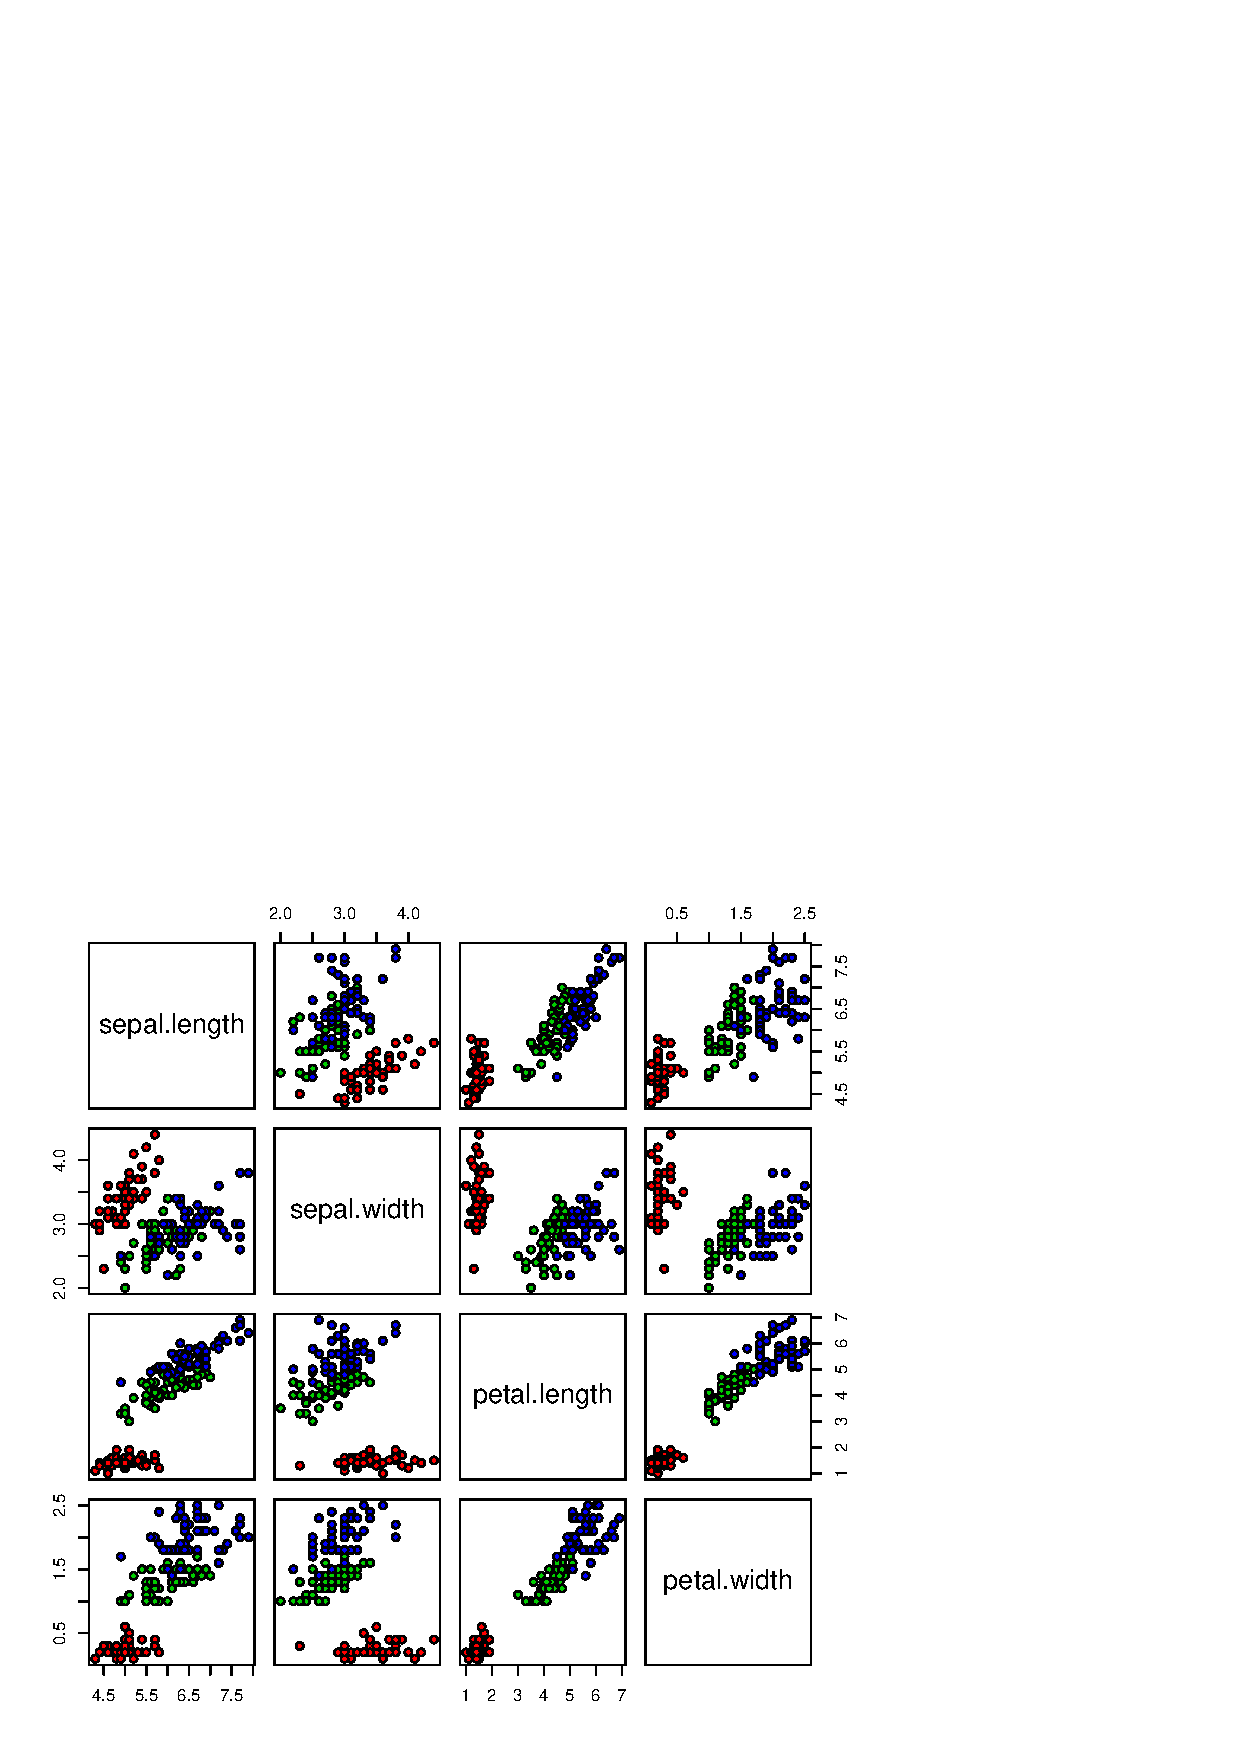
\includegraphics[width=0.8\textwidth]{images/ml/iris-flower-dataset}
  \end{center}
  \caption{Визуализация набора данных ``Ирисы Фишера''. setosa — красный, versicolor — зелёный, virginica — синий.}
  \label{ml:fig:iris-dataset-visualization}
\end{figure}
